% ============================================================
%  DISCOVERY CURRICULUM — Journey 4, Module 1
%  "Vector Fields and the Geometry of Space"
%  Compile with: pdflatex J4_M1.tex  (run twice)
% ============================================================
\documentclass[12pt,a4paper]{article}
\usepackage[a4paper,top=2.5cm,bottom=2.5cm,left=2.8cm,right=2.8cm,headheight=15pt]{geometry}
\usepackage{amsmath,amssymb,amsthm}
\usepackage{xcolor}
\usepackage{mdframed}
\usepackage{enumitem}
\usepackage{tikz}
\usetikzlibrary{arrows.meta,calc,decorations.markings}
\usepackage{pgfplots}
\pgfplotsset{compat=1.18}
\usepackage{booktabs}
\usepackage{fancyhdr}
\usepackage{titlesec}
\usepackage{parskip}
\usepackage{hyperref}
\hypersetup{colorlinks=true,linkcolor=NavyBlue,urlcolor=NavyBlue}

\definecolor{NavyBlue}{HTML}{1A3A5C}
\definecolor{MidBlue}{HTML}{2E6DA4}
\definecolor{Gold}{HTML}{C8922A}
\definecolor{LightBlue}{HTML}{EBF2FA}
\definecolor{LightGold}{HTML}{FDF4E3}
\definecolor{DarkGrey}{HTML}{3A3A3A}
\definecolor{BoxGreen}{HTML}{E8F5E9}
\definecolor{SidebarGrey}{HTML}{F5F5F5}

\titleformat{\section}{\Large\bfseries\color{NavyBlue}}{}{0em}{}[{\color{MidBlue}\vspace{2pt}\rule{\linewidth}{1.5pt}}]
\titleformat{\subsection}{\large\bfseries\color{MidBlue}}{}{0em}{}

\pagestyle{fancy}\fancyhf{}
\fancyhead[L]{\small\color{DarkGrey}\textit{Discovery Curriculum}}
\fancyhead[R]{\small\color{DarkGrey}\textit{Journey 4 $\cdot$ Module 1}}
\fancyfoot[C]{\small\color{MidBlue}\thepage}
\renewcommand{\headrulewidth}{0.4pt}

\newmdenv[backgroundcolor=NavyBlue!7,linecolor=NavyBlue,linewidth=2pt,leftline=true,rightline=false,topline=false,bottomline=false,innerleftmargin=14pt,innerrightmargin=10pt,innertopmargin=10pt,innerbottommargin=10pt,skipabove=14pt,skipbelow=10pt]{puzzlebox}
\newmdenv[backgroundcolor=LightGold,linecolor=Gold,linewidth=2pt,leftline=true,rightline=false,topline=false,bottomline=false,innerleftmargin=14pt,innerrightmargin=10pt,innertopmargin=10pt,innerbottommargin=10pt,skipabove=14pt,skipbelow=10pt]{discoverybox}
\newmdenv[backgroundcolor=LightBlue,linecolor=MidBlue,linewidth=1.5pt,roundcorner=4pt,innerleftmargin=14pt,innerrightmargin=10pt,innertopmargin=10pt,innerbottommargin=10pt,skipabove=14pt,skipbelow=10pt]{namebox}
\newmdenv[backgroundcolor=BoxGreen,linecolor=DarkGrey!35,linewidth=1pt,roundcorner=4pt,innerleftmargin=14pt,innerrightmargin=10pt,innertopmargin=10pt,innerbottommargin=10pt,skipabove=14pt,skipbelow=10pt]{reflectionbox}
\newmdenv[backgroundcolor=SidebarGrey,linecolor=Gold,linewidth=1.2pt,leftline=true,rightline=false,topline=false,bottomline=false,innerleftmargin=12pt,innerrightmargin=10pt,innertopmargin=7pt,innerbottommargin=7pt,skipabove=10pt,skipbelow=10pt]{thought}

\newcounter{problem}
\newenvironment{problem}[1][]{\refstepcounter{problem}\par\vspace{6pt}\noindent\textbf{\color{MidBlue}Problem \theproblem}\ifx&#1&\else\ \textit{(#1)}\fi\textbf{.}\enskip}{\par\vspace{4pt}}
\newcounter{deepproblem}
\newenvironment{deepproblem}[1][]{\refstepcounter{deepproblem}\par\vspace{6pt}\noindent\textbf{\color{NavyBlue}$\bigstar$\ Deep Problem \thedeepproblem}\ifx&#1&\else\ \textit{(#1)}\fi\textbf{.}\enskip}{\par\vspace{4pt}}

\begin{document}

\thispagestyle{empty}
\begin{center}
{\small\color{MidBlue}\textbf{DISCOVERY CURRICULUM}\quad$\cdot$\quad\textbf{JOURNEY 4: FIELDS AND SPACE}}
\vspace{0.6cm}

{\color{NavyBlue}\rule{\linewidth}{2pt}}\vspace{0.5cm}

{\Huge\bfseries\color{NavyBlue}Module 1}\\[0.3cm]
{\LARGE\bfseries\color{MidBlue}Vector Fields and the Geometry of Space}\\[0.4cm]
{\color{Gold}\rule{0.4\linewidth}{1.2pt}}\\[0.4cm]
{\large\itshape\color{DarkGrey}
A scalar field assigns a number to every point.\\[0.15cm]
A vector field assigns a direction and magnitude.\\[0.15cm]
The interplay between them is classical physics.}

\vspace{1cm}
\begin{tabular}{rl}
\color{DarkGrey}\textbf{Journey}         & Journey 4 --- Fields and Space \\[4pt]
\color{DarkGrey}\textbf{Module}          & 1 of 6 \\[4pt]
\color{DarkGrey}\textbf{Prerequisites}   & Journey 2 (multivariable calculus); Journey 3 (linear maps) \\[4pt]
\color{DarkGrey}\textbf{You will discover} & Scalar and vector fields, gradient, divergence, curl, line integrals, conservative fields \\[4pt]
\color{DarkGrey}\textbf{Format}          & 8 problems $+$ 3 deep problems $\approx$ 13 pages \\
\end{tabular}
\vspace{1cm}

{\color{NavyBlue}\rule{\linewidth}{2pt}}
\end{center}

\vspace{0.5cm}
\noindent\textbf{Opening Journey 4.}
Journey~2 differentiated and integrated functions $f:\mathbb{R}^n\to\mathbb{R}$. Journey~3 studied linear maps between vector spaces. Journey~4 puts them together: it studies functions $\mathbf{F}:\mathbb{R}^3\to\mathbb{R}^3$ --- vector fields --- and the three differential operators acting on them: gradient, divergence, and curl. These operators are the language in which all of classical physics is written. Maxwell's equations are four statements about vector fields. Newton's law of gravitation is a statement about a vector field. Fluid mechanics is the study of a velocity vector field.

\newpage

\section{Part 1 \texorpdfstring{---}{--} The Puzzle}

\begin{puzzlebox}
\textbf{The Opening Puzzle.}

A river flows through a valley. At each point $(x,y)$ in the valley, the water has a velocity $\mathbf{F}(x,y) = (-y, x)$.

\medskip
\textbf{Question 1.} Sketch this vector field by drawing $\mathbf{F}$ at the points $(\pm 1, 0)$, $(0,\pm 1)$, $(1,1)$, $(-1,1)$. What shape does the flow trace?

\textbf{Question 2.} A leaf is placed at $(1,0)$ at time $t=0$. Write and solve the ODE $\dot{\mathbf{r}} = \mathbf{F}(\mathbf{r})$ to find the leaf's path. What curve does it trace?

\textbf{Question 3.} A second leaf is placed at $(0,0)$. What happens to it? Why?

\textbf{Question 4.} How much work does the flow do on a leaf that travels once around the unit circle? Set up $\oint_C \mathbf{F}\cdot d\mathbf{r}$ and compute it.

\textbf{Question 5.} Compute $\frac{\partial F_y}{\partial x} - \frac{\partial F_x}{\partial y}$ for this field. What does this number measure geometrically?
\end{puzzlebox}

\section{Part 2 \texorpdfstring{---}{--} Exploration}

\subsection{Step 1: Scalar and vector fields}

\begin{problem}
\label{prob:fields_intro}
\begin{enumerate}[label=(\alph*),topsep=2pt]
  \item A \textbf{scalar field} assigns a real number to each point. Give three physical examples: one from thermodynamics, one from electrostatics, one from fluid mechanics.
  \item A \textbf{vector field} assigns a vector to each point. Give three physical examples: one force field, one velocity field, one from electromagnetism.
  \item The gradient $\nabla f = \left(\frac{\partial f}{\partial x}, \frac{\partial f}{\partial y}, \frac{\partial f}{\partial z}\right)$ is a vector field derived from a scalar field. Compute $\nabla f$ for $f(x,y,z) = x^2+y^2+z^2$ and describe the resulting vector field geometrically.
  \item Sketch the vector field $\mathbf{F}(x,y) = (x,y)$ (radially outward), $\mathbf{G}(x,y) = (-y,x)$ (rotational), and $\mathbf{H}(x,y) = (1,0)$ (uniform). Describe the qualitative character of each: is there a source, a rotation, a uniform flow?
  \item The \textbf{field lines} (integral curves) of a vector field $\mathbf{F}$ are curves $\mathbf{r}(t)$ satisfying $\dot{\mathbf{r}} = \mathbf{F}(\mathbf{r})$. Sketch the field lines of each field in (d). What determines their shape?
\end{enumerate}
\end{problem}

\begin{thought}
\textbf{Fields as the language of locality.}
Classical mechanics described forces between distant bodies: the Sun pulls the Earth across empty space. This troubled Newton himself --- it seemed to require ``action at a distance.'' Faraday's insight was that a charge does not directly pull another charge; instead, it creates a \emph{field} at every point in space, and the second charge responds to the local field at its own position. This localises physics: everything is determined by what is happening right here, right now. The field concept is one of the deepest shifts in the history of physics, and it is mathematically a function $\mathbf{F}:\mathbb{R}^3\to\mathbb{R}^3$. General relativity extends this: spacetime geometry is itself a field (the metric tensor field), and gravity is its curvature.
\end{thought}

\subsection{Step 2: Divergence and curl}

\begin{problem}
\label{prob:div_curl}
For $\mathbf{F} = (P,Q,R):\mathbb{R}^3\to\mathbb{R}^3$:
\[
  \nabla\cdot\mathbf{F} = \frac{\partial P}{\partial x}+\frac{\partial Q}{\partial y}+\frac{\partial R}{\partial z}, \qquad
  \nabla\times\mathbf{F} = \left(\frac{\partial R}{\partial y}-\frac{\partial Q}{\partial z},\; \frac{\partial P}{\partial z}-\frac{\partial R}{\partial x},\; \frac{\partial Q}{\partial x}-\frac{\partial P}{\partial y}\right).
\]
\begin{enumerate}[label=(\alph*),topsep=2pt]
  \item Compute $\nabla\cdot\mathbf{F}$ and $\nabla\times\mathbf{F}$ for:
    \begin{itemize}[noitemsep]
      \item $\mathbf{F}=(x,y,z)$ (radial)
      \item $\mathbf{G}=(-y,x,0)$ (rotational)
      \item $\mathbf{H}=(y^2z, 2xyz, xy^2)$
    \end{itemize}
  \item Show $\nabla\cdot(\nabla\times\mathbf{F})=0$ for any smooth $\mathbf{F}$ (the divergence of a curl is zero). This is an identity --- why?
  \item Show $\nabla\times(\nabla f)=\mathbf{0}$ for any smooth $f$ (the curl of a gradient is zero). This is also an identity.
  \item Interpret: $\nabla\cdot\mathbf{F}>0$ at a point means the field has a \emph{source} there (fluid flowing outward); $\nabla\cdot\mathbf{F}<0$ means a sink. $\nabla\times\mathbf{F}\neq\mathbf{0}$ means the field \emph{circulates} locally. A tiny paddlewheel placed in the fluid would rotate if $\nabla\times\mathbf{F}\neq\mathbf{0}$.
  \item Verify: the radial field $(x,y,z)/r^3$ (gravity and electrostatics) has $\nabla\cdot\mathbf{F}=0$ and $\nabla\times\mathbf{F}=\mathbf{0}$ everywhere except the origin. What is special about the origin?
\end{enumerate}
\end{problem}

\begin{center}
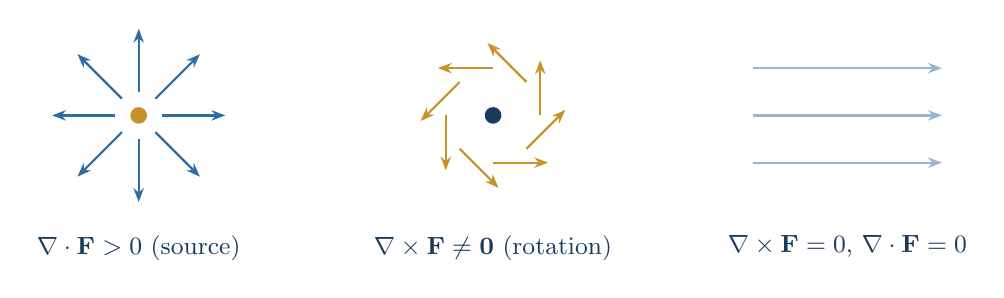
\begin{tikzpicture}
% Left: diverging field (source)
\begin{scope}[xshift=0cm]
\foreach \angle in {0,45,...,315}{
  \draw[-{Stealth[length=5pt]},MidBlue,thick]
    ({0.3*cos(\angle)},{0.3*sin(\angle)}) --
    ({1.1*cos(\angle)},{1.1*sin(\angle)});
}
\fill[Gold] (0,0) circle (3pt);
\node[below,font=\small,color=NavyBlue] at (0,-1.4) {$\nabla\cdot\mathbf{F}>0$ (source)};
\end{scope}
% Right: rotating field (curl)
\begin{scope}[xshift=4.5cm]
\foreach \angle in {0,45,...,315}{
  \pgfmathsetmacro{\px}{cos(\angle)}
  \pgfmathsetmacro{\py}{sin(\angle)}
  \pgfmathsetmacro{\vx}{-sin(\angle)*0.7}
  \pgfmathsetmacro{\vy}{cos(\angle)*0.7}
  \draw[-{Stealth[length=5pt]},Gold,thick]
    ({\px*0.6},{\py*0.6}) -- ({\px*0.6+\vx},{\py*0.6+\vy});
}
\fill[NavyBlue] (0,0) circle (3pt);
\node[below,font=\small,color=NavyBlue] at (0,-1.4) {$\nabla\times\mathbf{F}\neq\mathbf{0}$ (rotation)};
\end{scope}
% Right: irrotational, source-free
\begin{scope}[xshift=9cm]
\foreach \i in {-1,0,1}{
  \draw[-{Stealth[length=5pt]},MidBlue!50,thick]
    (-1.2,{\i*0.6}) -- (1.2,{\i*0.6});
}
\node[below,font=\small,color=NavyBlue] at (0,-1.4) {$\nabla\times\mathbf{F}=0$, $\nabla\cdot\mathbf{F}=0$};
\end{scope}
\end{tikzpicture}
\end{center}

\subsection{Step 3: Line integrals and work}

\begin{problem}
\label{prob:line_int}
The \textbf{line integral} $\int_C\mathbf{F}\cdot d\mathbf{r}$ measures the work done by $\mathbf{F}$ along the curve $C$.

\begin{enumerate}[label=(\alph*),topsep=2pt]
  \item Parametrise $C$ as $\mathbf{r}(t)$, $a\leq t\leq b$. Write $\int_C\mathbf{F}\cdot d\mathbf{r} = \int_a^b\mathbf{F}(\mathbf{r}(t))\cdot\mathbf{r}'(t)\,dt$.
  \item Compute $\int_C\mathbf{F}\cdot d\mathbf{r}$ for $\mathbf{F}=(y,-x)$ along: (i) the upper semicircle from $(1,0)$ to $(-1,0)$; (ii) the straight line from $(1,0)$ to $(-1,0)$. Are the two values equal?
  \item Compute $\int_C\mathbf{G}\cdot d\mathbf{r}$ for $\mathbf{G}=(2x, 2y)$ along both paths from (b). Are the two values equal this time?
  \item A \textbf{conservative field} is one where $\int_C\mathbf{F}\cdot d\mathbf{r}$ depends only on the endpoints, not the path. Show that $\mathbf{G}=(2x,2y)$ is conservative by finding a scalar potential $\phi$ with $\nabla\phi = \mathbf{G}$.
  \item Show: $\mathbf{F}$ is conservative if and only if $\oint_C\mathbf{F}\cdot d\mathbf{r}=0$ for every closed loop $C$. Verify for both fields above.
\end{enumerate}
\end{problem}

\begin{problem}
\label{prob:conservative}
\textbf{When is a field conservative?}
\begin{enumerate}[label=(\alph*),topsep=2pt]
  \item Show: if $\mathbf{F}=\nabla\phi$, then $\nabla\times\mathbf{F}=\mathbf{0}$ (curl-free $\Rightarrow$ conservative). This follows from $\nabla\times(\nabla\phi)=\mathbf{0}$.
  \item The converse: if $\nabla\times\mathbf{F}=\mathbf{0}$ on a \emph{simply connected} domain, then $\mathbf{F}=\nabla\phi$ for some $\phi$. Verify this is false on $\mathbb{R}^2\setminus\{0\}$ for $\mathbf{F}=\frac{(-y,x)}{x^2+y^2}$: compute $\nabla\times\mathbf{F}$ (it's zero) but compute $\oint\mathbf{F}\cdot d\mathbf{r}$ around the unit circle (it's $2\pi\neq 0$). What topological property of the domain matters?
  \item Find the potential function for $\mathbf{F}=(yz, xz, xy)$. (Check $\nabla\times\mathbf{F}=\mathbf{0}$ first, then integrate.)
  \item In classical mechanics, a \textbf{conservative force} is $\mathbf{F}=-\nabla V$ (gradient of negative potential energy). Show that the work done by a conservative force equals the decrease in potential energy. This is conservation of energy.
  \item Gravity near Earth: $\mathbf{F}=(0,0,-mg)$. Find the potential $V$. Show the work done lifting a mass from height $h_1$ to $h_2$ equals $mg(h_2-h_1)$, independent of path.
\end{enumerate}
\end{problem}

\subsection{Step 4: Surface integrals and flux}

\begin{problem}
\label{prob:flux}
The \textbf{flux} of $\mathbf{F}$ through a surface $S$ is $\iint_S\mathbf{F}\cdot d\mathbf{A} = \iint_S\mathbf{F}\cdot\hat{\mathbf{n}}\,dA$, where $\hat{\mathbf{n}}$ is the unit normal.

\begin{enumerate}[label=(\alph*),topsep=2pt]
  \item Interpret: flux measures how much of $\mathbf{F}$ passes through $S$ per unit time (for a fluid velocity field).
  \item Compute the flux of $\mathbf{F}=(x,y,z)$ through the unit sphere $S:\, x^2+y^2+z^2=1$ outward. Parametrise using spherical coordinates $x=\sin\phi\cos\theta$, $y=\sin\phi\sin\theta$, $z=\cos\phi$.
  \item Compute the flux of the uniform field $\mathbf{F}=(1,0,0)$ through the unit sphere. Interpret physically: why is the net flux zero?
  \item For the gravitational field $\mathbf{F}=-\frac{GM}{r^3}\mathbf{r}$ (where $\mathbf{r}=(x,y,z)$, $r=|\mathbf{r}|$): compute the outward flux through a sphere of radius $R$ centred at the origin. Does the answer depend on $R$?
  \item The answer to (d) is independent of $R$. What does this tell you physically? (Hint: think about what is inside the sphere.)
\end{enumerate}
\end{problem}

\begin{problem}
\label{prob:operators_summary}
The three differential operators and their relationships:
\begin{enumerate}[label=(\alph*),topsep=2pt]
  \item Write the three operators in terms of the symbolic vector $\nabla = (\partial_x, \partial_y, \partial_z)$: gradient $= \nabla f$; divergence $= \nabla\cdot\mathbf{F}$; curl $= \nabla\times\mathbf{F}$.
  \item Compute the \textbf{Laplacian} $\nabla^2 f = \nabla\cdot(\nabla f) = \partial_x^2 f + \partial_y^2 f + \partial_z^2 f$ for $f=x^2+y^2-2z^2$ and $g=x^2+y^2+z^2$.
  \item A function satisfying $\nabla^2 f=0$ is \textbf{harmonic}. Show $f=x^2-y^2$ is harmonic in 2D. Give the physical context where harmonic functions arise.
  \item In spherical coordinates, the Laplacian is $\nabla^2 f = \frac{1}{r^2}\frac{\partial}{\partial r}\left(r^2\frac{\partial f}{\partial r}\right) + \frac{1}{r^2\sin\phi}\frac{\partial}{\partial\phi}\left(\sin\phi\frac{\partial f}{\partial\phi}\right) + \frac{1}{r^2\sin^2\phi}\frac{\partial^2 f}{\partial\theta^2}$. Verify $\nabla^2(1/r)=0$ for $r\neq 0$. This is the fundamental solution of the Laplace equation.
  \item Connect: $\nabla\times(\nabla f) = \mathbf{0}$ and $\nabla\cdot(\nabla\times\mathbf{F}) = 0$ are both instances of the identity $d^2=0$ in differential forms (from Journey~2, Module~6 deep problem). Write one sentence explaining the pattern.
\end{enumerate}
\end{problem}

\section{Part 3 \texorpdfstring{---}{--} Discovery}

\begin{discoverybox}
\textbf{What have we built?}

\textbf{First.} Scalar fields (temperature, potential, pressure) and vector fields (force, velocity, electric field) are the fundamental objects of classical physics. The differential operators $\nabla$, $\nabla\cdot$, $\nabla\times$ measure how they vary in space.

\textbf{Second.} Divergence measures local source strength; curl measures local rotation. A field with zero curl on a simply connected domain has a scalar potential; a field with zero divergence has a vector potential.

\textbf{Third.} Line integrals measure work; surface integrals measure flux. Conservative fields are those for which line integrals are path-independent --- they are gradients of scalar potentials, and they encode conservation of energy.

\textbf{Fourth.} The identities $\nabla\times(\nabla f)=\mathbf{0}$ and $\nabla\cdot(\nabla\times\mathbf{F})=\mathbf{0}$ are instances of $d^2=0$, connecting to the differential forms of Journey~2 and the topology of the domain.

\medskip
\textbf{The pattern.} The sequence $f \xrightarrow{\nabla} \mathbf{F} \xrightarrow{\nabla\times} \mathbf{G} \xrightarrow{\nabla\cdot} h$ has the property that successive operators compose to zero: $\nabla\times(\nabla f)=\mathbf{0}$ and $\nabla\cdot(\nabla\times\mathbf{F})=\mathbf{0}$. This is a \emph{complex} in the sense of homological algebra. Module~2 will show this complex is exact (no wasted kernel) and prove the great integral theorems.
\end{discoverybox}

\section{Part 4 \texorpdfstring{---}{--} Naming the Ideas}

\begin{namebox}
\textbf{Vector calculus operators.}

$\nabla f = \left(\partial_x f,\partial_y f,\partial_z f\right)$ (\textbf{gradient}): points uphill, perpendicular to level surfaces.

$\nabla\cdot\mathbf{F} = \partial_x P+\partial_y Q+\partial_z R$ (\textbf{divergence}): measures outward flux per unit volume.

$\nabla\times\mathbf{F} = (\partial_y R-\partial_z Q,\, \partial_z P-\partial_x R,\, \partial_x Q-\partial_y P)$ (\textbf{curl}): measures circulation per unit area.

$\nabla^2 f = \nabla\cdot(\nabla f)$ (\textbf{Laplacian}): measures deviation of $f$ from its local average.

\textbf{Key identities}: $\nabla\times(\nabla f)=\mathbf{0}$;\quad $\nabla\cdot(\nabla\times\mathbf{F})=0$.
\end{namebox}

\begin{namebox}
\textbf{Conservative fields.}

$\mathbf{F}$ is \textbf{conservative} iff any of these equivalent conditions hold: $\oint_C\mathbf{F}\cdot d\mathbf{r}=0$ for all closed $C$; $\mathbf{F}=\nabla\phi$ for some scalar potential $\phi$; $\nabla\times\mathbf{F}=\mathbf{0}$ (on a simply connected domain).

The work-energy theorem: work done by $\mathbf{F}=-\nabla V$ equals $-\Delta V$ (decrease in potential energy).
\end{namebox}

\section{Part 5 \texorpdfstring{---}{--} Deep Problems}

\begin{deepproblem}[The Helmholtz decomposition]
Every smooth vector field $\mathbf{F}$ on a simply connected domain can be decomposed as
\[
  \mathbf{F} = -\nabla\phi + \nabla\times\mathbf{A},
\]
where $\phi$ is a scalar potential and $\mathbf{A}$ is a vector potential.
\begin{enumerate}[label=(\alph*)]
  \item The first term is \textbf{curl-free} (irrotational); the second is \textbf{divergence-free} (solenoidal). Show this.
  \item In electrostatics, $\mathbf{E} = -\nabla\phi$ (electric field from scalar potential). In magnetostatics, $\mathbf{B} = \nabla\times\mathbf{A}$ (magnetic field from vector potential). Show that Maxwell's equations $\nabla\cdot\mathbf{B}=0$ and $\nabla\times\mathbf{E}=0$ (static case) are automatically satisfied by these potentials.
  \item \textbf{Gauge freedom}: the potentials $\phi$ and $\mathbf{A}$ are not unique. Show that replacing $\phi\to\phi-\partial_t\chi$ and $\mathbf{A}\to\mathbf{A}+\nabla\chi$ (gauge transformation) leaves $\mathbf{E}$ and $\mathbf{B}$ unchanged.
  \item The \textbf{Coulomb gauge} fixes $\nabla\cdot\mathbf{A}=0$. Show that under this condition $\phi$ satisfies the Poisson equation $\nabla^2\phi = -\rho/\varepsilon_0$.
\end{enumerate}
\end{deepproblem}

\begin{deepproblem}[Topology and the failure of Poincaré's lemma]
Poincaré's lemma states: on a simply connected domain, every curl-free field is a gradient (and every divergence-free field is a curl).
\begin{enumerate}[label=(\alph*)]
  \item Show that $\mathbf{F} = \frac{(-y,x,0)}{x^2+y^2}$ has $\nabla\times\mathbf{F}=\mathbf{0}$ on $\mathbb{R}^3\setminus\{z\text{-axis}\}$, but $\oint_C\mathbf{F}\cdot d\mathbf{r} = 2\pi$ for any loop $C$ linking the $z$-axis. Conclude: $\mathbf{F}$ is not a gradient.
  \item The fundamental group $\pi_1(X)$ of a space $X$ counts the essentially different loops. $\pi_1(\mathbb{R}^2\setminus\{0\}) = \mathbb{Z}$ (loops classified by winding number). Show the winding number of $C$ around the origin equals $\frac{1}{2\pi}\oint_C\mathbf{F}\cdot d\mathbf{r}$.
  \item The de Rham cohomology $H^1(\mathbb{R}^2\setminus\{0\}) = \mathbb{R}$ is generated by $\mathbf{F}$. It measures the failure of closed forms to be exact. Connect this to the result in Journey~2 Module~6 deep problem 3.
  \item \textit{(Research.)} Aharonov-Bohm effect: an electron passes around a solenoid (region of confined $\mathbf{B}$). Outside the solenoid, $\mathbf{B}=\mathbf{0}$ but $\mathbf{A}\neq\mathbf{0}$. The electron's quantum phase shifts by $\frac{e}{\hbar}\oint\mathbf{A}\cdot d\mathbf{r}$, producing an observable interference pattern even though the electron never enters the magnetic field. This is a physical measurement of de Rham cohomology. Describe the experiment in one paragraph.
\end{enumerate}
\end{deepproblem}

\begin{deepproblem}[The Laplacian and harmonic functions]
\begin{enumerate}[label=(\alph*)]
  \item The \textbf{mean value property}: if $f$ is harmonic on a domain containing a ball $B(P,r)$, then $f(P)$ equals the average of $f$ on the sphere $\partial B(P,r)$. Accept this (it follows from Green's identities). Deduce the \textbf{maximum principle}: a harmonic function cannot attain its maximum in the interior of its domain.
  \item The maximum principle implies uniqueness of the Dirichlet problem: if $\nabla^2 f=0$ in a domain $\Omega$ and $f=g$ on $\partial\Omega$, then $f$ is uniquely determined. Prove this: if $f_1$ and $f_2$ are both solutions, consider $u=f_1-f_2$.
  \item The function $f(x,y) = \text{Re}(z^n)$ where $z=x+iy$ is harmonic for any $n$. Verify for $n=2$ (giving $f=x^2-y^2$) and $n=3$ (giving $f=x^3-3xy^2$). What is the connection between harmonic functions and complex analysis?
  \item \textbf{Green's first identity}: $\int_\Omega u\nabla^2v\,dV = \oint_{\partial\Omega}u\nabla v\cdot d\mathbf{A} - \int_\Omega\nabla u\cdot\nabla v\,dV$. Prove this using the divergence theorem applied to $u\nabla v$. Derive Green's second identity (symmetric version).
  \item Use Green's first identity with $u=v=f$ (harmonic) to prove $\int_\Omega|\nabla f|^2\,dV = \oint_{\partial\Omega}f\frac{\partial f}{\partial n}\,dA$. Interpret: the energy of a harmonic field is determined entirely by its boundary values.
\end{enumerate}
\end{deepproblem}

\section{Part 6 \texorpdfstring{---}{--} Reflection}

\begin{reflectionbox}
\textbf{Your reflection task.}

\begin{enumerate}
  \item \textbf{On fields.} Before fields, physics was about particles and forces between them. After Faraday and Maxwell, physics was about fields that fill all of space. Write a paragraph: does the field picture feel more or less fundamental than particles? What would it mean for a field to be the \emph{primary} physical reality, with particles as secondary phenomena?

  \item \textbf{On conservation of energy.} We showed that conservative forces satisfy $\mathbf{F}=-\nabla V$, and that work equals $-\Delta V$. This is conservation of energy --- but only for conservative forces. Where does the energy go for non-conservative forces (e.g.\ friction)? Is energy actually conserved in those cases at a deeper level?

  \item \textbf{On the identities.} The identities $\nabla\times\nabla f=0$ and $\nabla\cdot(\nabla\times\mathbf{F})=0$ are purely algebraic consequences of the symmetry of mixed partial derivatives. Yet they encode profound physical content (there are no magnetic monopoles; the circulation of a conservative field is zero). Write one sentence on how an algebraic identity can carry physical meaning.

  \item \textbf{Looking ahead.} Module~2 proves the integral theorems: Gauss, Stokes, and Green. You saw these in Journey~2 Module~6 in a brief preview. Now you have the language to prove them and understand their physical content. Before the module: state what you expect Gauss's theorem to say in terms of divergence and flux, and Stokes' theorem in terms of curl and circulation.
\end{enumerate}
\end{reflectionbox}

\medskip
\noindent\textbf{Looking ahead.}
Module~2 proves the three great integral theorems --- Gauss, Stokes, Green --- that connect local information (divergence and curl) to global information (flux and circulation). These are the backbone of all of classical physics: Maxwell's equations in integral form are four applications of these theorems.

\vspace{1.4cm}
\begin{center}
{\color{MidBlue}\rule{0.5\linewidth}{0.8pt}}\\[6pt]
{\small\color{DarkGrey}\textit{End of Journey 4, Module 1 --- Vector Fields and the Geometry of Space}}\\[4pt]
{\small\color{DarkGrey}Continue to: \textbf{Module 2 --- The Integral Theorems}}\\[6pt]
{\color{MidBlue}\rule{0.5\linewidth}{0.8pt}}
\end{center}

\end{document}